\chapter{Tables and Images}
\label{ch:third_chapter}
This chapter contains examples of large tables and grid-arranged images.

\section{1x3 Grid}
Here is an example of an image grid, as shown in Figure \ref{fig:fruit_images1x3}.
\begin{figure}[h!]
\centering

\begin{subfigure}[t]{0.30\textwidth}
  \centering
  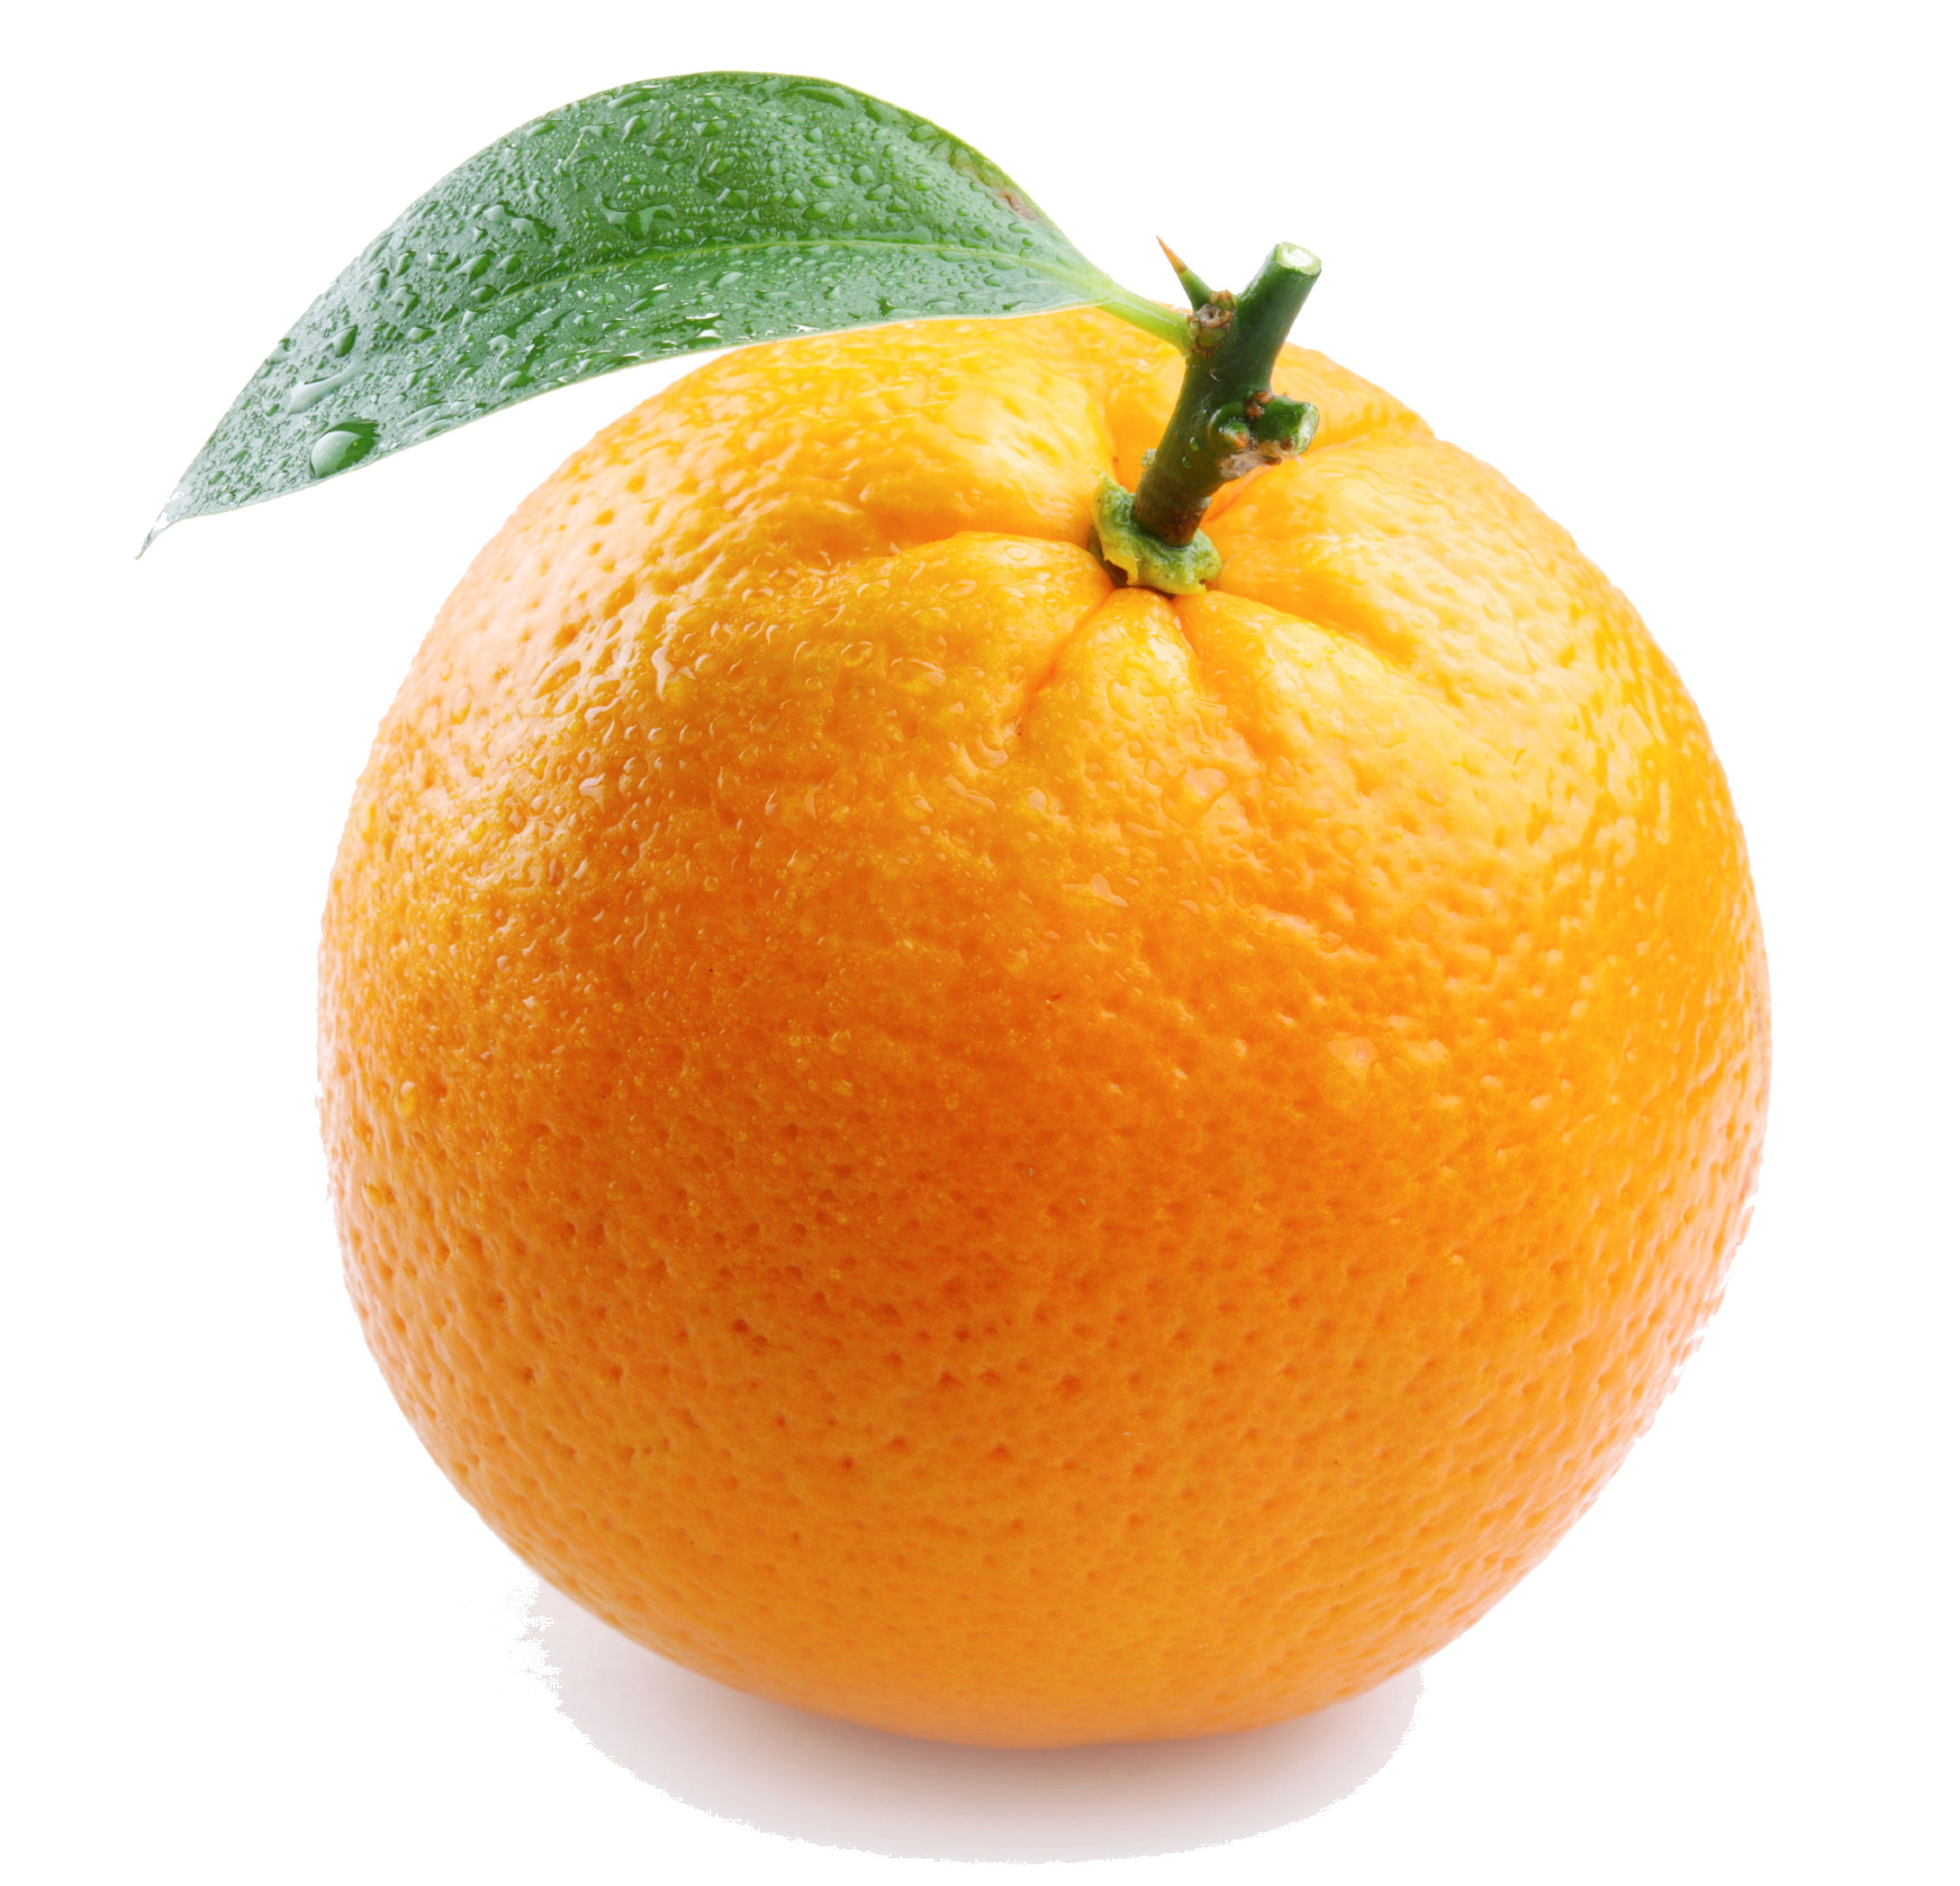
\includegraphics[width=\linewidth]{images/fruits/arancia.jpg}
  \caption{Orange}
\end{subfigure}\hfill
\begin{subfigure}[t]{0.30\textwidth}
  \centering
  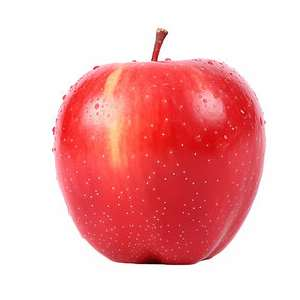
\includegraphics[width=\linewidth]{images/fruits/mela.jpg}
  \caption{Apple}
\end{subfigure}\hfill
\begin{subfigure}[t]{0.30\textwidth}
  \centering
  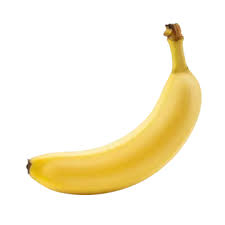
\includegraphics[width=\linewidth]{images/fruits/banana.jpg}
  \caption{Banana}
\end{subfigure}

\caption{Photos of fresh fruit in a 1x3 grid.}
\label{fig:fruit_images1x3}
\end{figure}

\section{2x2 Grid}
Here is an example of an image grid, as shown in Figure \ref{fig:fruit_images2x2}.
\begin{figure}[H]
\centering

% --- First row ---
\begin{subfigure}[t]{0.45\textwidth}
  \centering
  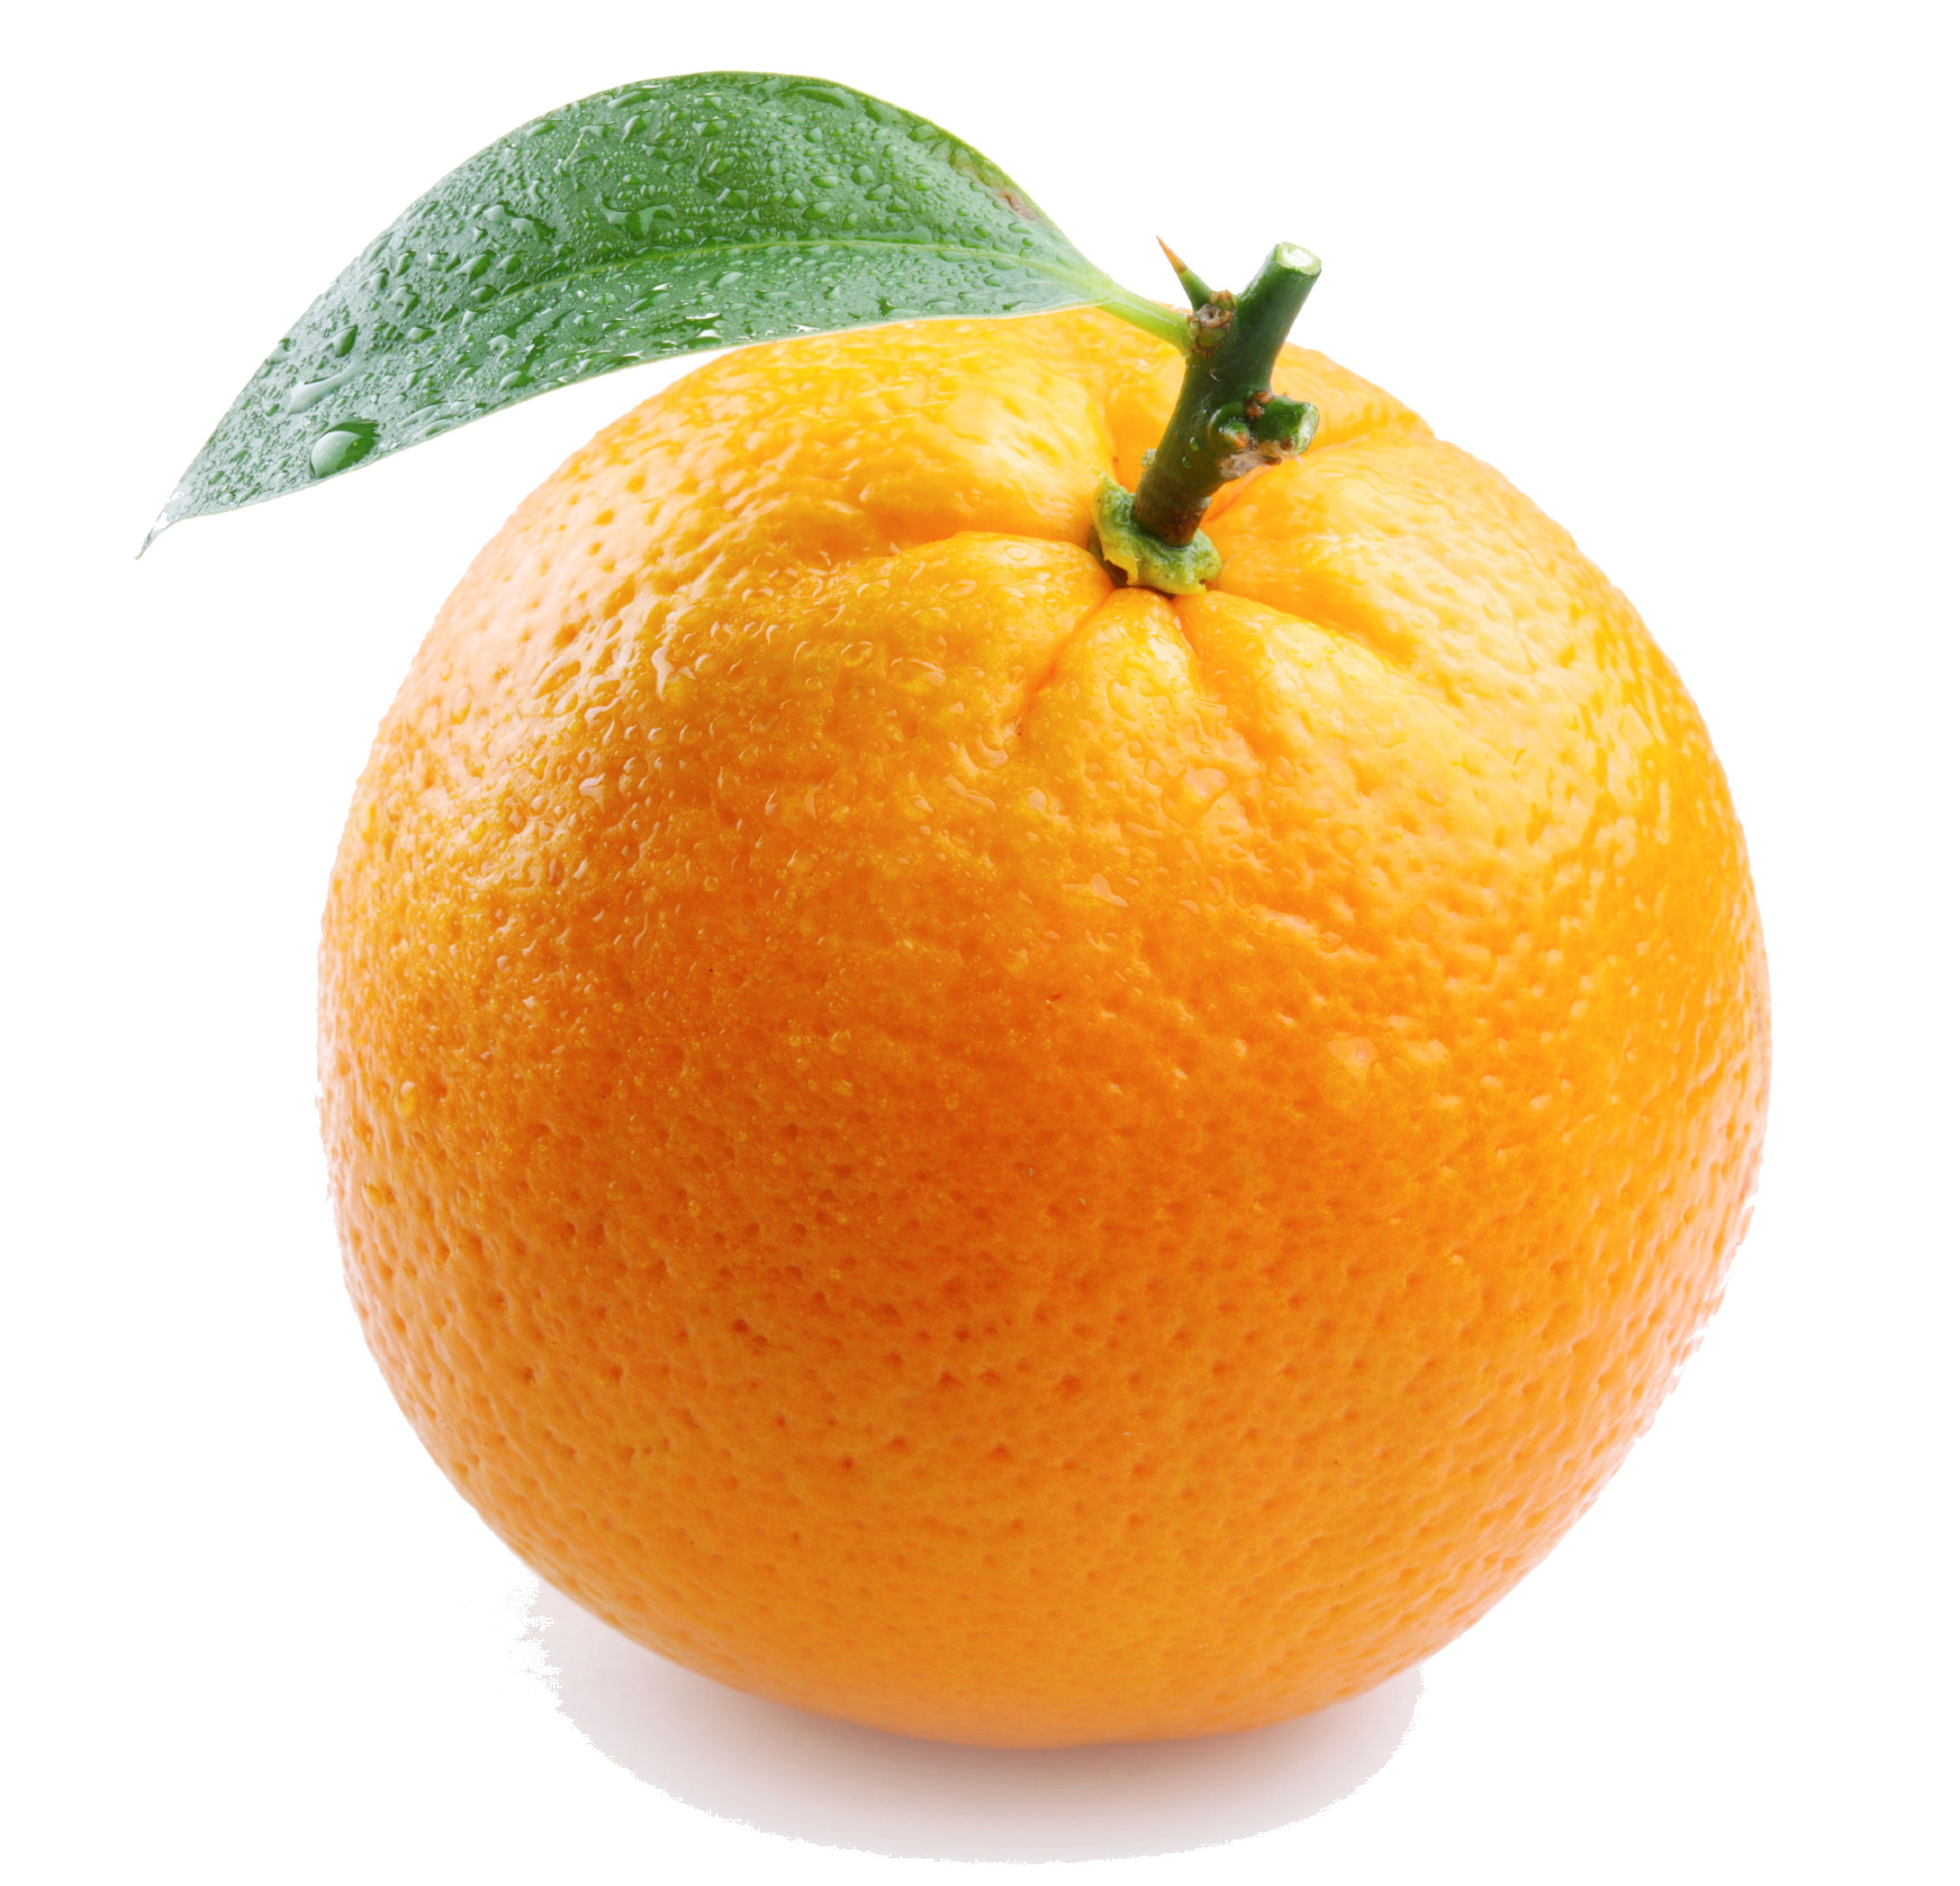
\includegraphics[width=\linewidth]{images/fruits/arancia.jpg}
  \caption{Orange}
\end{subfigure}\hfill
\begin{subfigure}[t]{0.45\textwidth}
  \centering
  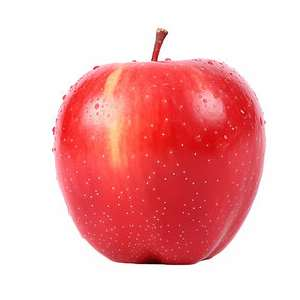
\includegraphics[width=\linewidth]{images/fruits/mela.jpg}
  \caption{Apple}
\end{subfigure}

% --- Second row ---
\begin{subfigure}[t]{0.45\textwidth}
  \centering
  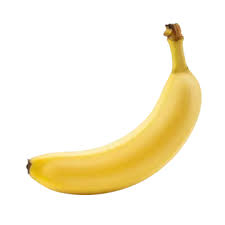
\includegraphics[width=\linewidth]{images/fruits/banana.jpg}
  \caption{Banana}
\end{subfigure}\hfill
\begin{subfigure}[t]{0.45\textwidth}
  \centering
  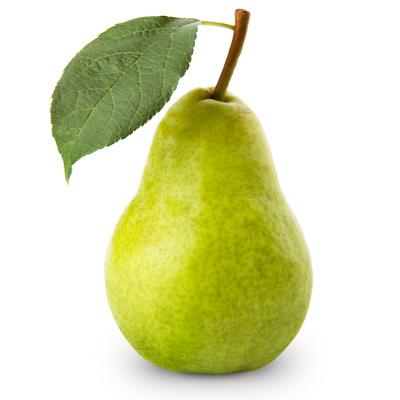
\includegraphics[width=\linewidth]{images/fruits/pera.jpg}
  \caption{Pear}
\end{subfigure}

\caption{Photos of fresh fruit in a 2×2 grid.}
\label{fig:fruit_images2x2}
\end{figure}

\section{Example of a Complex Table}
\input{tables/complex_table}
